% SC4242 --- Chapter 7: Register Allocation & Code Generation (0->100 ground-up)
\chapter{Register Allocation and Code Generation}
\label{ch:regalloc}

\begin{quote}
\emph{``Infinite virtual registers, $k$ physical ones: colour the interference graph or spill.''} --- Then tile trees to select instructions and honour the calling convention.
\end{quote}

\noindent\fbox{\parbox{\dimexpr\linewidth-2\fboxsep-2\fboxrule}{%
\textbf{From zero: we build here, no backend assumed.} We define target instructions, calling convention, liveness, interference, graph colouring, spilling, linear scan, and instruction selection from sets/graphs. Pictures precede algorithms.}}
\vspace{0.4em}

\section*{Learning Outcomes}
After this chapter you will be able to:
\begin{enumerate}[label=(L\arabic*)]
    \item compute liveness intervals and build the interference graph;
    \item colour the graph via Chaitin--Briggs (simplify, spill, select) and coalesce moves;
    \item spill with reloads, estimate spill cost, and iterate;
    \item contrast graph colouring vs.\ linear scan and pick per target;
    \item tile IR trees for instruction selection (maximal munch / DP) and emit correct prologue/epilogue.
\end{enumerate}

% ============================================================
\section{Why Registers Are Scarce}
\label{sec:why-regs}
\emph{Intuition:} IR uses unbounded temporaries $t_1,t_2,\dots$; a real CPU has $k$ general-purpose registers (e.g., $k=16$ on x86-64, $32$ on ARM, but fewer caller-saved). Two temporaries \emph{interfere} if both live at some point---they cannot share a register. The problem is graph colouring.

\begin{definition}[Liveness for intervals]
For CFG in SSA or after SSA destruction, $t$ is \emph{live} at point $p$ if a path $p\to use(t)$ has no intervening def. Its \emph{live interval} $[def(t), last\_use(t)]$ over linear order (after block linearisation) conservatively covers where it interferes. Exact interference is per-program-point, not just interval (holes where $t$ not live inside interval are okay to reuse if using graph, not linear scan).
\end{definition}

\begin{example}[Intervals for \texttt{a=b+c*2}]
3AC: $t_1=c*2$, $t_2=b+t_1$, $a=t_2$. Linear order: 1:\texttt{t1}, 2:\texttt{t2}, 3:\texttt{a}. Live: $c$ live at 1, $b$ live at 2, $t_1$ live $1\to2$, $t_2$ live $2\to3$. So $b$ interferes with $t_1$ (both live at 2? $b$ used at 2, $t_1$ live through 2), but $c$ not with $t_2$.
\end{example}

% TikZ 1: live intervals + interference graph
\begin{figure}[h]
\centering
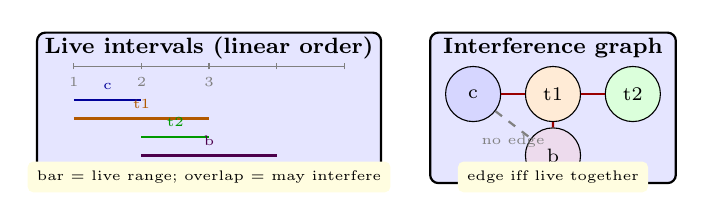
\begin{tikzpicture}[scale=0.78,every node/.style={font=\scriptsize}]
% intervals
\draw[thick,fill=blue!10,rounded corners=3pt] (0,0) rectangle (5.6,2.45);
\node[font=\footnotesize\bfseries] at (2.8,2.20) {Live intervals (linear order)};
\draw[gray,thin] (0.6,1.9)--(5.0,1.9);
\foreach \x in {0.6,1.7,2.8,3.9,5.0} {\draw[gray,thin] (\x,1.85)--(\x,1.95);}
\node[font=\tiny,gray] at (0.6,1.65) {1};
\node[font=\tiny,gray] at (1.7,1.65) {2};
\node[font=\tiny,gray] at (2.8,1.65) {3};
\draw[thick,blue!60!black] (0.6,1.35)--(1.7,1.35) node[midway,above,font=\tiny] {c};
\draw[thick,orange!70!black] (0.6,1.05)--(2.8,1.05) node[midway,above,font=\tiny] {t1};
\draw[thick,green!60!black] (1.7,0.75)--(2.8,0.75) node[midway,above,font=\tiny] {t2};
\draw[thick,violet!60!black] (1.7,0.45)--(3.9,0.45) node[midway,above,font=\tiny] {b};
% legend
\node[font=\tiny,fill=yellow!12,rounded corners=2pt] at (2.8,0.10) {bar = live range; overlap = may interfere};
% interference graph
\begin{scope}[xshift=6.4cm]
\draw[thick,fill=blue!10,rounded corners=3pt] (0,0) rectangle (4.0,2.45);
\node[font=\footnotesize\bfseries] at (2.0,2.20) {Interference graph};
\node[draw,circle,fill=blue!16,minimum size=0.7cm] (n1) at (0.7,1.45) {c};
\node[draw,circle,fill=orange!16,minimum size=0.7cm] (n2) at (2.0,1.45) {t1};
\node[draw,circle,fill=green!14,minimum size=0.7cm] (n3) at (3.3,1.45) {t2};
\node[draw,circle,fill=violet!14,minimum size=0.7cm] (n4) at (2.0,0.45) {b};
\draw[thick,red!60!black] (n1)--(n2);
\draw[thick,red!60!black] (n2)--(n4);
\draw[thick,red!60!black] (n2)--(n3);
\draw[thick,dashed,gray] (n1)--(n4) node[midway,below,font=\tiny] {no edge};
\node[font=\tiny,fill=yellow!12,rounded corners=2pt] at (2.0,0.10) {edge iff live together};
\end{scope}
\end{tikzpicture}
\caption{Live intervals over linearised blocks (left) induce the interference graph (right). Graph colouring is precise; linear scan uses only interval overlap and may over-approximate.}
\label{fig:intervals-interf}
\end{figure}

% ============================================================
\section{Graph Colouring Allocation (Chaitin--Briggs)}
\label{sec:chaitin}
\emph{Intuition:} $k$-colour the graph where $k$ = register count. If degree $<k$, a node can always be coloured after neighbours (remove it, colour rest, then pick a free colour). If all degrees $\ge k$, pick a spill candidate, spill it to stack, and retry.

\paragraph{Briggs optimistic variant.} Simplify: repeatedly remove any node with degree $<k$ onto stack (if none, pick spill candidate by cost heuristic $uses+defs$ weighted by loop depth $10^{depth}$, push it optimistically anyway). Then select: pop stack, assign first colour not used by already-coloured neighbours; if none, this node is the actual spill---insert reload before each use and store after each def, rewrite, and repeat.

\paragraph{Coalescing.} Move $x\gets y$ where $x,y$ do not interfere can be coalesced (same register, move deleted) if the merged node stays $<k$-colourable (Briggs: combined neighbours $<k$ high-degree neighbours). Iterative coalescing interleaves simplify/coalesce for best elimination.

\begin{example}[4-colour walkthrough with spill]
Graph: $\{\text{t1--c, t1--b, t1--t2, a--t2}\}$ plus many neighbours. With $k=2$ registers, simplify removes $c,a$ (degree $1$), leaving core $\{t1,b,t2\}$ where each degree $2$ ($=k$)---no $<k$ node. Pick spill least cost, say $b$ (cold). Stack $[c,a,b,t1,t2]$; selecting colours: $t2\to R0$, $t1$ interferes $t2$ so $R1$, $b$ interferes $t1$ so $R0$ (optimistically coloured---no spill needed!). If all 3 had pairwise edges (triangle) with $k=2$, the last popped \emph{would} spill and be reloaded from stack slot.
\end{example}

% TikZ 2: colouring and spill illustration
\begin{figure}[h]
\centering
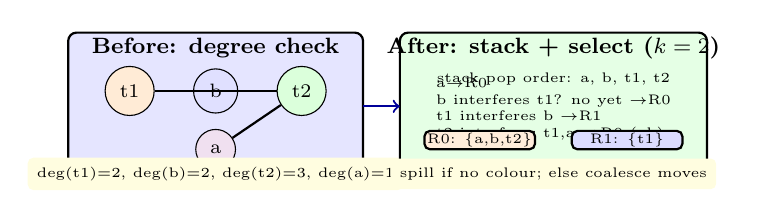
\begin{tikzpicture}[scale=0.78,every node/.style={font=\scriptsize}]
% before
\begin{scope}
\draw[thick,fill=blue!10,rounded corners=3pt] (0,0) rectangle (4.8,2.45);
\node[font=\footnotesize\bfseries] at (2.4,2.20) {Before: degree check};
\node[draw,circle,fill=orange!16] (a) at (1.0,1.5) {t1};
\node[draw,circle,fill=blue!12] (b) at (2.4,1.5) {b};
\node[draw,circle,fill=green!14] (c) at (3.8,1.5) {t2};
\node[draw,circle,fill=violet!12] (d) at (2.4,0.55) {a};
\draw[thick] (a)--(b); \draw[thick] (a)--(c); \draw[thick] (b)--(c); \draw[thick] (c)--(d);
\node[font=\tiny,fill=yellow!12,rounded corners=2pt] at (2.4,0.15) {deg(t1)=2, deg(b)=2, deg(t2)=3, deg(a)=1};
\end{scope}
\begin{scope}[xshift=5.4cm]
\draw[thick,fill=green!10,rounded corners=3pt] (0,0) rectangle (5.0,2.45);
\node[font=\footnotesize\bfseries] at (2.5,2.20) {After: stack + select ($k=2$)};
\node[font=\tiny,align=left] at (2.5,1.70) {stack pop order: a, b, t1, t2};
\node[font=\tiny,align=left] at (2.5,1.20) {a$\to$R0\\ b interferes t1? no yet $\to$R0\\ t1 interferes b $\to$R1\\ t2 interferes t1,a $\to$R0 (ok)};
\draw[thick,fill=orange!14,rounded corners=2pt] (0.4,0.55) rectangle (2.2,0.85);
\node[font=\tiny] at (1.3,0.70) {R0: \{a,b,t2\}};
\draw[thick,fill=blue!14,rounded corners=2pt] (2.8,0.55) rectangle (4.6,0.85);
\node[font=\tiny] at (3.7,0.70) {R1: \{t1\}};
\node[font=\tiny,fill=yellow!12,rounded corners=2pt] at (2.5,0.15) {spill if no colour; else coalesce moves};
\end{scope}
\draw[->,thick,blue!60!black] (4.8,1.25)--(5.4,1.25);
\end{tikzpicture}
\caption{Briggs simplify/select with $k=2$: remove low-degree nodes, then assign colours on the way back. Spill only if truly needed; coalescing would merge a move-related pair if safe.}
\label{fig:colouring}
\end{figure}

\begin{lstlisting}[language=Python]
def colour(interf, k, move_pairs):
    stack, removed = [], set()
    # simplify + coalesce loop
    while len(stack)+len(removed) < len(interf):
        v = pick_low_degree(interf, removed, k) or pick_spill(interf, removed)
        stack.append(v); removed.add(v)
        coalesce_around(v, interf, move_pairs, k)
    colour_of = {}
    spilled = set()
    while stack:
        v = stack.pop()
        used = {colour_of[w] for w in interf[v] if w in colour_of}
        free = [c for c in range(k) if c not in used]
        if free: colour_of[v]=free[0]
        else: spilled.add(v)          # insert spill code and retry
    return colour_of, spilled
\end{lstlisting}

% ============================================================
\section{Linear Scan and Instruction Selection}
\label{sec:linear-scan}
\paragraph{Linear scan (Poletto--Sarkar).} Sort intervals by start; sweep maintaining \emph{active} intervals (those overlapping current start). If $|\text{active}|=k$, spill the interval with farthest end (or current if it ends farthest---then current spills, not active). Fast $O(n\log n)$, used by JITs (HotSpot, V8) where compile speed beats last-percent quality. Holes are ignored (pessimistic).

\paragraph{Instruction selection by tiling.} IR tree (e.g., $+(b,*(c,2))$) is tiled with target patterns: $c*2\to\texttt{sll }c,1$ (strength reduce), $b+t_1\to\texttt{add}$. Maximal-munch picks largest tile greedily; optimal DP picks min-cost cover (BURS). Fig.~\ref{fig:tiling} shows tiling.

% TikZ 3: linear scan intervals + tiling
\begin{figure}[h]
\centering
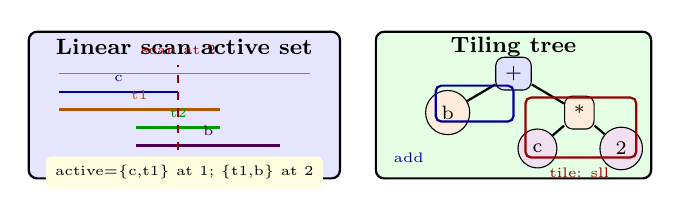
\begin{tikzpicture}[scale=0.76,every node/.style={font=\scriptsize}]
% linear scan
\draw[thick,fill=blue!10,rounded corners=3pt] (0,0) rectangle (5.2,2.45);
\node[font=\footnotesize\bfseries] at (2.6,2.20) {Linear scan active set};
\draw[gray,thin] (0.5,1.75)--(4.7,1.75);
\draw[thick,blue!60!black] (0.5,1.45)--(2.5,1.45) node[midway,above,font=\tiny] {c};
\draw[thick,orange!70!black] (0.5,1.15)--(3.2,1.15) node[midway,above,font=\tiny] {t1};
\draw[thick,green!60!black] (1.8,0.85)--(3.2,0.85) node[midway,above,font=\tiny] {t2};
\draw[thick,violet!60!black] (1.8,0.55)--(4.2,0.55) node[midway,above,font=\tiny] {b};
\draw[thick,dashed,red!60!black] (2.5,0.2)--(2.5,1.9) node[above,font=\tiny] {scan at 2};
\node[font=\tiny,fill=yellow!12,rounded corners=2pt] at (2.6,0.10) {active=\{c,t1\} at 1; \{t1,b\} at 2};
% tiling
\begin{scope}[xshift=5.8cm]
\draw[thick,fill=green!10,rounded corners=3pt] (0,0) rectangle (4.6,2.45);
\node[font=\footnotesize\bfseries] at (2.3,2.20) {Tiling tree};
\node[draw,fill=blue!12,rounded corners=3pt] (r) at (2.3,1.75) {+};
\node[draw,fill=orange!14,circle] (b) at (1.2,1.1) {b};
\node[draw,fill=orange!14,rounded corners=3pt] (m) at (3.4,1.1) {*};
\node[draw,fill=violet!12,circle] (c) at (2.7,0.5) {c};
\node[draw,fill=violet!12,circle] (k) at (4.1,0.5) {2};
\draw[thick] (r)--(b); \draw[thick] (r)--(m); \draw[thick] (m)--(c); \draw[thick] (m)--(k);
\draw[thick,red!60!black,rounded corners=2pt] (2.5,0.35) rectangle (4.35,1.35);
\node[font=\tiny,red!60!black] at (3.4,0.10) {tile: sll};
\draw[thick,blue!60!black,rounded corners=2pt] (2.3,1.55) rectangle (1.0,0.95);
\node[font=\tiny,blue!60!black] at (0.55,0.35) {add};
\end{scope}
\end{tikzpicture}
\caption{Left: linear scan sweep with active set; spill farthest-ending. Right: IR tree $b+(c*2)$ tiled as \texttt{sll} for $c*2$ plus \texttt{add} for $b+t_1$. Cost DP chooses minimal tiles.}
\label{fig:tiling}
\end{figure}

\paragraph{Calling convention \& prologue/epilogue.} Caller-saved vs.\ callee-saved registers, argument registers ($a0$--$a3$ on MIPS, $r0$--$r3$ on ARM), return $v0$, stack alignment (16B), and spill slots all emitted in function prologue (\texttt{push ra, fp; sub sp, framesize}) and epilogue. Correctness requires spilled temps reload before every use.

\begin{lstlisting}[language=C]
// MIPS-like emitter after allocation: R0 -> $t0, R1 -> $t1
// 3AC: t1 = c * 2; t2 = b + t1; a = t2  with t1->R1, b->R1? conflict so b->R0
lw $t0, b          // b in R0
lw $t1, c          // c in R1
sll $t1, $t1, 1    // t1 = c*2  (tiling picked sll)
add $t0, $t0, $t1  // t2 reuses $t0
sw $t0, a
\end{lstlisting}

% ============================================================
\section{Chapter Notes}
Chaitin (1982) cast allocation as colouring; Briggs (1992) made it optimistic with coalescing; George--Appel refined iterated coalescing. Linear scan (Poletto--Sarkar 1999) trades a few percent runtime for 10$\times$ compile speed---why JITs love it. Tiling theory is Aho--Johnson (1976) and Fraser--Hanson (BURG). For ARM/x86 specifics, consult ABI docs and Appel Ch.~10--11.

% ============================================================
\section{Exercises}
\label{sec:ch07-exercises}
\begin{enumerate}[label=E7.\arabic*, leftmargin=*, itemsep=0.8em]
\item \textbf{Interf from liveness.} CFG with blocks B1:\texttt{x=1}, B2:\texttt{y=x+2}, B3:\texttt{z=x+y}, edges B1$\to$B2,B3, B2$\to$B3. Compute LiveIn/Out, then interference edges. Which pairs interfere? Why does interval approximation add a false edge?
\item \textbf{Briggs on triangle.} Graph $K_3$ (3 nodes clique) with $k=2$. Simulate simplify: degree $<2$? none, pick spill cheapest, push, stack, then select and show one node must spill. What spill code inserted? Second iteration?
\item \textbf{Coalescing safety.} Move \texttt{a=b} with interference edges a--c, b--c only, $k=2$. Is coalescing a,b safe by Briggs criterion (combined high-degree neighbours $<k$)? Show merged graph and colour it with 2 colours, move gone.
\item \textbf{Linear scan spill choice.} Intervals: a$[1,4)$, b$[2,3)$, c$[2,6)$, d$[5,7)$ with $k=2$. Sweep sorted by start: at 2 active \{a\} size 1 add b $\to$2, add c $\to$3$>k$ so spill farthest end (c ends 6 vs a 4 vs b 3: spill c). Trace full sweep and final mapping.
\item \textbf{Tiling DP.} IR tree $(b+c)*(d+2)$ with patterns: add$\to$\texttt{add} cost 1, mul$\to$\texttt{mul} cost 2, mul by 2$\to$\texttt{sll} cost 1. Compute minimal tile cost via DP (postorder: leaf cost 0, plus pattern). Which mul becomes sll?
\end{enumerate}
% End of Chapter 7
